\chapter{THE MARSHALL-OLKIN DISTRIBUTION}\label{chap:MO}
%%%%%%%%%%%%%%%%%%%%%%%%%%%%%%%%%%%%%%%%%%%%%%%%%%%%%%%%%%%%%%%%%%%%%%%%%%%%%%%%%%%%%
%%%%%%%%%%%%%%%%%%%%%%%%%%%%%%%%%%%%%%%%%%%%%%%%%%%%%%%%%%%%%%%%%%%%%%%%%%%%%%%%%%%%%
%%%%%%%%%%%%%%%%%%%%%%%%%%%%%%%%%%%%%%%%%%%%%%%%%%%%%%%%%%%%%%%%%%%%%%%%%%%%%%%%%%%%%
%%%%%%%%%%%%%%%%%%%%%%%%%%%%%%%%%%%%%%%%%%%%%%%%%%%%%%%%%%%%%%%%%%%%%%%%%%%%%%%%%%%%%
%%%%%%%%%%%%%%%%%%%%%%%%%%%%%%%%%%%%%%%%%%%%%%%%%%%%%%%%%%%%%%%%%%%%%%%%%%%%%%%%%%%%%
\section{Introducing the Marshall-Olkin Distribution}
\hspace{24pt} Albert W. Marshall and Ingram Olkin introduced the Marshall-Olkin (MO) distribution in 1967. They claimed that they were the first to have proposed a multivariate exponential distribution with an applicable use. This distribution arises from ``shock models" and its ability to model the failing of a two-component system \cite{marshallolkin1967}. Define three independent random variables, where $Z_1\sim\text{Exp}\left(\lambda_1\right)$, $Z_2\sim\text{Exp}\left(\lambda_2\right)$, and $Z_3\sim\text{Exp}\left(\lambda_3\right)$ represent the time until occurrences of the shocks. The first two random variables are shocks to component one and component two, respectively, and the last random variable is a shock to both components. Now define two random variables $X=\min\{Z_1,Z_3\}$ and $Y=\min\{Z_2,Z_3\}$. These new random variables represent the lifetimes of component one and component two, respectively. We can now find the joint survival function. The survival function will allow for more convenient calculations than working with the joint CDF.
\begin{align*}
    S_{X,Y}\left(x,y\right)&=P\left(X>x,Y>y\right)\\
    &=P\left(\min\{Z_1,Z_3\}>x,\min\{Z_2,Z_3\}>y\right)\\
    &=P\left(Z_1>x,Z_3>x,Z_2>y,Z_3>y\right)\\
    &=P\left(Z_1>x,Z_2>y,Z_3>\max\{x,y\}\right)\\
    &=\exp\left\{-\left(\lambda_1x+\lambda_2y+\lambda_3\max\{x,y\}\right)\right\},\qquad x,y>0
\end{align*}
The visual of an exponential distribution curve is very well known. However, the MO distribution is difficult to visualize because of the ``max" term. Let's show an example with three different sets of parameters.
\begin{figure}[ht]
    \centering
    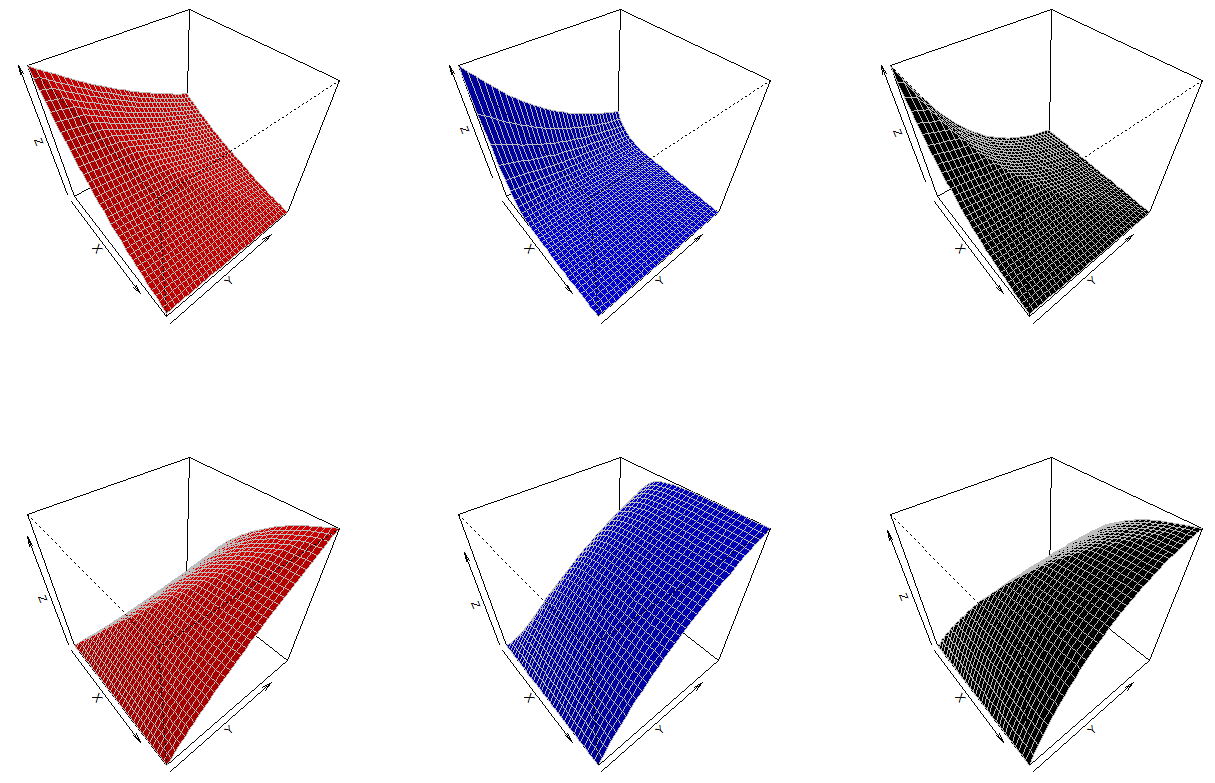
\includegraphics[scale=0.45]{images/3DMO.PNG}
    %\caption{The red graph shows $\lambda_1=1$, $\lambda_2=0.2$, and $\lambda_3=0.5$. The blue graph shows $\lambda_1=10$, $\lambda_2=1$, and $\lambda_3=0.5$. The black graph shows $\lambda_1,=0.5$, $\lambda_2=0.5$, $\lambda_3=2$. The top row shows the survival function and the bottom row shows the CDF.}
    \caption{The red graph shows $\lambda_1=1$, $\lambda_2=0.2$, and $\lambda_3=0.5$; the blue graph shows $\lambda_1=10$, $\lambda_2=1$, and $\lambda_3=0.5$; the black graph shows $\lambda_1,=0.5$, $\lambda_2=0.5$, $\lambda_3=2$; the top row shows the survival function and the bottom row shows the CDF.}
    \label{fig:MO3d}
\end{figure}
%%%%%%%%%%%%%%%%%%%%%%%%%%%%%%%%%%%%%%%%%%%%%%%%%%%%%%%%%%%%%%%%%%%%%%%%%%%%%%%%%%%%%
%%%%%%%%%%%%%%%%%%%%%%%%%%%%%%%%%%%%%%%%%%%%%%%%%%%%%%%%%%%%%%%%%%%%%%%%%%%%%%%%%%%%%
%%%%%%%%%%%%%%%%%%%%%%%%%%%%%%%%%%%%%%%%%%%%%%%%%%%%%%%%%%%%%%%%%%%%%%%%%%%%%%%%%%%%%
%%%%%%%%%%%%%%%%%%%%%%%%%%%%%%%%%%%%%%%%%%%%%%%%%%%%%%%%%%%%%%%%%%%%%%%%%%%%%%%%%%%%%
%%%%%%%%%%%%%%%%%%%%%%%%%%%%%%%%%%%%%%%%%%%%%%%%%%%%%%%%%%%%%%%%%%%%%%%%%%%%%%%%%%%%%
\section{Rank Correlation of the Marshall-Olkin Distribution}
\hspace{24pt} The population definitions have been defined in multiple ways for both Spearman's Rho and Kendall's Tau. We can now use them to define these rank correlation methods for the MO distribution. We will begin with Spearman's Rho, because for Kendall's Tau we have to invoke a Lemma that will be defined soon.
\begin{theorem}\label{theorem:MOrho}
    Spearman's Rho for the Marshall-Olkin distribution can be defined as $$\rho_S=\frac{3\alpha_1\alpha_2}{2\alpha_1+2\alpha_2-\alpha_1\alpha_2}$$ where $\alpha_1=\frac{\lambda_3}{\lambda_1+\lambda_3}$ and $\alpha=\frac{\lambda_3}{\lambda_2+\lambda_3}$.
\end{theorem}
\begin{proof}
    Recall Theorem \ref{theorem:rho}, where Spearman's Rho is defined as $$Q\left(C,\Pi\right)=12\int\int_{[0,1]^2}C\left(u,v\right)\mathrm{d}u\mathrm{d}v-3.$$ We can use this definition by finding the copula for the MO distribution. To find the copula, make the following observations. Notice that $\max\left\{x,y\right\}=x+y-\min\left\{x,y\right\}$. The marginal survival functions for $X$ and $Y$ are $S_X\left(x\right)=\exp\left\{-\left(\lambda_1+\lambda_3\right)x\right\}$ and $S_Y\left(y\right)=\exp\left\{-\left(\lambda_2+\lambda_3\right)y\right\}$, respectively. To make future calculations easier, let $\alpha_1=\frac{\lambda_3}{\lambda_1+\lambda_3}$ and $\alpha_2=\frac{\lambda_3}{\lambda_2+\lambda_3}$. Using these observations, we will start with the survival function, manipulate it, then apply the copula transformation.
    \begin{align*}
        S_{X,Y}\left(x,y\right)&=\exp\left\{-\left(\lambda_1x+\lambda_2y+\lambda_3\max\left\{x,y\right\}\right)\right\}\\
        &=\exp\left\{-\left(\lambda_1+\lambda_3\right)x-\left(\lambda_2+\lambda_3\right)y+\lambda_3\min\left\{x,y\right\}\right\}\\
        &=\exp\left\{-\left(\lambda_1+\lambda_3\right) x\right\}\exp\left\{-\left(\lambda_2+\lambda_3\right)y\right\}\exp\left\{\lambda_3\min\left\{x,y\right\}\right\}\\
        &=S_X\left(x\right)S_Y\left(y\right)\min\left\{\exp\left\{\lambda_3x\right\},\;\exp\left\{\lambda_3y\right\}\right\}
    \end{align*}
    Using the fact that $\exp\left\{\lambda_3x\right\}=S_X\left(x\right)^{-\alpha_1}$ and $\exp\left\{\lambda_3y\right\}=S_Y\left(y\right)^{-\alpha_2}$, now apply the copula transformation $U=F_X\left(x\right)$, $V=F_Y\left(y\right)$. Let $\overline{C}$ be the survival copula.
    \begin{align*}
        \overline{C}\left(u,v\right)&=u\, v\min\left\{u^{-\alpha_1},v^{-\alpha_2}\right\}\\
        &=\min\left\{v\, u^{1-\alpha_1},u\, v^{1-\alpha_2}\right\}\\
        &=\begin{cases}v\, u^{1-\alpha_1} & ,u^{\alpha_1}\geq v^{\alpha_2}\\ u\, v^{1-\alpha_2} & ,u^{\alpha_1}\leq v^{\alpha_2}\\ \end{cases}
    \end{align*}
    The MO distribution contains a singular component. This is a concentrated cluster of density on the line $y=x$ (or the line $u^{\alpha_1}=v^{\alpha_2}$). Because of this, the integral in Theorem \ref{theorem:rho} will have to be split into two parts to account for this cluster. To visualize this, consider Figure \ref{fig:MOsim} below, a simulation done using the software R. Now that the copula has been defined, apply to Theorem \ref{theorem:rho}.
    \begin{figure}
        \centering
        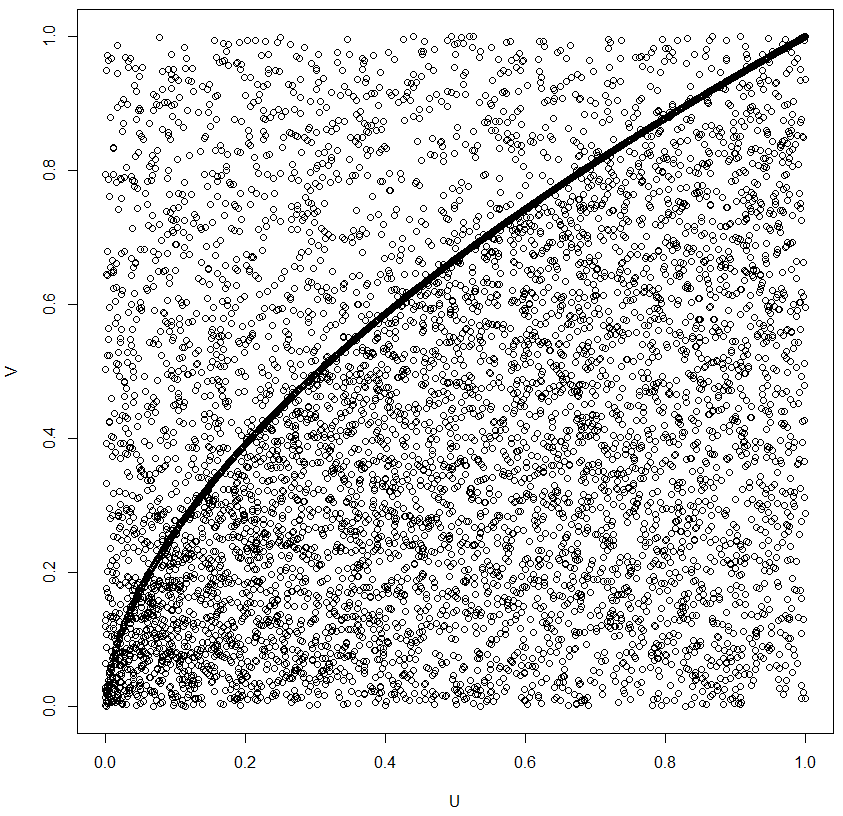
\includegraphics[scale=0.6]{images/MOsimulation.PNG}
        %\caption{Simulation of the Marshall-Olkin survival copula using parameters: $\lambda_1=0.7$, $\lambda_2=0.2$, and $\lambda_3=0.5$. The simulation is done in the open-source software R.}
        \caption{Simulation of the Marshall-Olkin survival copula using parameters: $\lambda_1=0.7$, $\lambda_2=0.2$, and $\lambda_3=0.5$.}
        \label{fig:MOsim}
    \end{figure}
    \begin{align*}
        \rho_S&=12\int\int_{[0,1]^2}C\left(u,v\right)\mathrm{d}u\mathrm{d}v-3\\
        &=12\int_0^1\left[\int_0^{u^{\alpha_1/\alpha_2}}v\, u^{1-\alpha_1}\mathrm{d}v+\int_{u^{\alpha_1/\alpha_2}}^1u\, v^{1-\alpha_2}\mathrm{d}v\right]\mathrm{d}u-3\\
        &=12\int_0^1\left[u^{1-\alpha_1}\frac{1}{2}v^2\bigg|_0^{u^{\alpha_1/\alpha_2}}+u\, \frac{v^{2-\alpha_2}}{2-\alpha_2}\bigg|_{u^{\alpha_1/\alpha_2}}^1\right]\mathrm{d}u-3\\
        &=12\int_0^1\left[\frac{u^{1-\alpha_1}u^{2\alpha_1/\alpha_2}}{2}+\left(\frac{u}{2-\alpha_2}-\frac{u\, u^{\left(\alpha_1/\alpha_2\right)\left(2-\alpha_2\right)}}{2-\alpha_2}\right)\right]\mathrm{d}u-3\\
        &=12\int_0^1\left[u^{2\alpha_1/\alpha_2-\alpha_1+1}\left(\frac{1}{2}-\frac{1}{2-\alpha_2}\right)+\frac{u}{2-\alpha_2}\right]\mathrm{d}u-3\\
        &=12\left[\left(\frac{1}{2}-\frac{1}{2-\alpha_2}\right)\frac{u^{2\alpha_1/\alpha_2-\alpha_1+2}}{2\alpha_1/\alpha_2-\alpha_1+2}\bigg|_0^1+\frac{u^2}{2\left(2-\alpha_2\right)}\bigg|_0^1\right]-3\\
        &=12\left[\left(\frac{1}{2}-\frac{1}{2-\alpha_2}\right)\left(\frac{1}{2\alpha_1/\alpha_2-\alpha_1+2}\right)+\frac{1}{2\left(2-\alpha_2\right)}\right]-3\\
        &=12\left[\frac{2-\alpha_2-2+2\alpha_1/\alpha_2-\alpha_1+2}{2\left(2-\alpha_2\right)\left(2\alpha_1/\alpha_2-\alpha_1+2\right)}\right]-3\\
        &=\frac{-12\alpha_2+24\alpha_1/\alpha_2-12\alpha_1+24}{2\left(2-\alpha_2\right)\left(2\alpha_1/\alpha_2-\alpha_1+2\right)}-\frac{6\left(2-\alpha_2\right)\left(2\alpha_1\alpha_2-\alpha_1+2\right)}{2\left(2-\alpha_2\right)\left(2\alpha_1/\alpha_2-\alpha_1+2\right)}\\
        &=\frac{12\alpha_1-6\alpha_1\alpha_2}{2\left(2-\alpha_2\right)\left(2\alpha_1/\alpha_2-\alpha_1+2\right)}\\
        &=\frac{3\alpha_1}{2\alpha_1/\alpha_2-\alpha_1+2}\\
        &=\frac{3\alpha_1\alpha_2}{2\alpha_1+2\alpha_2-\alpha_1\alpha_2}
    \end{align*}
    In terms of lambda, we can define it as $$\rho_S=\frac{3\left(\frac{\lambda_3}{\lambda_1+\lambda_3}\right)\left(\frac{\lambda_3}{\lambda_2+\lambda_3}\right)}{2\left(\frac{\lambda_3}{\lambda_1+\lambda_3}\right)+2\left(\frac{\lambda_3}{\lambda_2+\lambda_3}\right)-\left(\frac{\lambda_3}{\lambda_1+\lambda_3}\right)\left(\frac{\lambda_3}{\lambda_2+\lambda_3}\right)}$$
\end{proof}
For the Kendall's Tau definition of the MO distribution, we will take the same route as Spearman's Rho by using the copula. We will first define a lemma to help us evaluate integrals with singular components. The original lemma was proved by Li, X. in 2002 \cite{li2002} in terms of copulas. Here, we state it in terms of CDFs.
\begin{lemma}\label{lem:li}
    Let $F_{X,Y}\left(x,y\right)$ and $G_{X,Y}\left(x,y\right)$ be differentiable CDFs. Then $$\int\int_{\mathbb{R}^2}F_{X,Y}\left(x,y\right)\mathrm{d}G_{X,Y}\left(x,y\right)=\frac{1}{2}-\int\int_{\mathbb{R}^2}\frac{\partial}{\partial x}F_{X,Y}\left(x,y\right)\frac{\partial}{\partial y}G_{X,Y}\left(x,y\right)\mathrm{d}x\mathrm{d}y.$$
\end{lemma}
Using Lemma \ref{lem:li}, we will now derive Kendall's Tau for the MO distribution.
\begin{theorem}\label{theorem:MOtau}
    Kendall's Tau for the Marshall-Olkin distribution can be derived as $$\tau=\frac{\alpha_1\alpha_2}{\alpha_1+\alpha_2-\alpha_1\alpha_2}$$ where $\alpha_1=\frac{\lambda_3}{\lambda_1+\lambda_3}$ and $\alpha=\frac{\lambda_3}{\lambda_2+\lambda_3}$.
\end{theorem}
\begin{proof}
    \begin{align*}
        \tau&=4\int\int_{[0,1]^2}C\left(u,v\right)\mathrm{d}C\left(u,v\right)-1\\
        &=4\left[\frac{1}{2}-\int\int_{[0,1]^2}\frac{\partial}{\partial u}C\left(u,v\right)\frac{\partial}{\partial v}C\left(u,v\right)\mathrm{d}u\mathrm{d}v\right]-1\\
        &=4\left[\frac{1}{2}-\int_0^1\left(\int_0^{u^{\alpha_1/\alpha_2}}\frac{\partial}{\partial u}u^{1-\alpha_1}v\frac{\partial}{\partial v}u^{1-\alpha_1}v\mathrm{d}v+\int_{u^{\alpha_1/\alpha_2}}^1\frac{\partial}{\partial u}uv^{1-\alpha_2}\frac{\partial}{\partial v}uv^{1-\alpha_2}\mathrm{d}v\right)\mathrm{d}u\right]-1\\
        &=4\left[\frac{1}{2}-\int_0^1\left(\int_0^{u^{\alpha_1/\alpha_2}}\left(1-\alpha_1\right)u^{-\alpha_1}vu^{1-\alpha_1}\mathrm{d}v-\int_{u^{\alpha_1/\alpha_2}}^1uv^{1-\alpha_2}\left(1-\alpha_2\right)v^{-\alpha_2}\mathrm{d}v\right)\mathrm{d}u\right]-1\\
        &=4\left[\frac{1}{2}-\int_0^1\left(\frac{1-\alpha_1}{2}u^{1-2\alpha_1}v^2\bigg|_0^{u^{\alpha_1/\alpha_2}}+\frac{1-\alpha_2}{2-2\alpha_2}uv^{2-2\alpha_2}\bigg|_{u^{\alpha_1/\alpha_2}}^1\right)\mathrm{d}u\right]-1\\
        &=4\left[\frac{1}{2}-\int_0^1\left(\frac{1-\alpha_1}{2}u^{2\alpha_1/\alpha_2-2\alpha_1+1}+\frac{1}{2}u-\frac{1}{2}u^{2\alpha_1/\alpha_2-2\alpha_1+1}\right)\mathrm{d}u\right]-1\\
        &=2\left(1+\alpha_1\frac{u^{2\alpha_1/\alpha_2-2\alpha_1+2}}{2\alpha_1/\alpha_2-2\alpha_1+2}\bigg|_0^1-\frac{1}{2}u^2\bigg|_0^1\right)-1\\
        &=2\left(1+\frac{\alpha_1}{2\alpha_1/\alpha_2-2\alpha_1+2}-\frac{1}{2}\right)-1\\
        &=\frac{\alpha_1}{\alpha_1/\alpha_2-\alpha_1+1}\\
        &=\frac{\alpha_1\alpha_2}{\alpha_1+\alpha_2-\alpha_1\alpha_2}
    \end{align*}
    In terms of lambda, we can define it as $$\tau=\frac{\left(\frac{\lambda_3}{\lambda_1+\lambda_3}\right)\left(\frac{\lambda_3}{\lambda_2+\lambda_3}\right)}{\frac{\lambda_3}{\lambda_1+\lambda_3}+\frac{\lambda_3}{\lambda_2+\lambda_3}+\left(\frac{\lambda_3}{\lambda_1+\lambda_3}\right)\left(\frac{\lambda_3}{\lambda_2+\lambda_3}\right)}$$
\end{proof}
For both of the previous proofs we could have arrived at the same solutions by using the CDF versions. We now have all the information we need to find the bias of the Marshall-Olkin distribution in terms of the mixing proportion, $p$.
%%%%%%%%%%%%%%%%%%%%%%%%%%%%%%%%%%%%%%%%%%%%%%%%%%%%%%%%%%%%%%%%%%%%%%%%%%%%%%%%%%%%%
%%%%%%%%%%%%%%%%%%%%%%%%%%%%%%%%%%%%%%%%%%%%%%%%%%%%%%%%%%%%%%%%%%%%%%%%%%%%%%%%%%%%%
%%%%%%%%%%%%%%%%%%%%%%%%%%%%%%%%%%%%%%%%%%%%%%%%%%%%%%%%%%%%%%%%%%%%%%%%%%%%%%%%%%%%%
%%%%%%%%%%%%%%%%%%%%%%%%%%%%%%%%%%%%%%%%%%%%%%%%%%%%%%%%%%%%%%%%%%%%%%%%%%%%%%%%%%%%%
%%%%%%%%%%%%%%%%%%%%%%%%%%%%%%%%%%%%%%%%%%%%%%%%%%%%%%%%%%%%%%%%%%%%%%%%%%%%%%%%%%%%%
\section{Bias of Rank Correlation Under a Mixture Model}\label{sec:MObias}
\hspace{24pt} Consider two populations that follow a bivariate Marshall-Olkin distribution, one being a valid population and the other contaminating. Define the parameters for each to be $$\left(X,Y\right)_V\sim\text{MO}\left(\lambda_{V1},\lambda_{V2},\lambda_{V3}\right)\qquad\text{and}\qquad\left(X,Y\right)_C\sim\text{MO}\left(\lambda_{C1},\lambda_{C2},\lambda_{C3}\right).$$
To find the bias in terms of the mixing proportion we can anticipate there will be a lot of integrals to solve in order to arrive at the desired analytical solution. However, by noticing a pattern for each integral in the coefficients from Theorem \ref{theorem:main} we can formulate a general integral to solve. This is because each integral follows a similar form, the only difference being valid or contaminated survival function. Furthermore, some of the integrals are equivalent to the ones solved in both Theorem \ref{theorem:MOrho} and \ref{theorem:MOtau}. Recall the bias from Theorem \ref{theorem:main}, $$\text{Bias}_{\tau}\left(p\right)=\tau_{\vec{M}}-\tau_{\vec{V}}=4\left(a_{\tau}p^2+b_{\tau}p\right)$$ where
\begin{align*}
    a_\tau=&\int\int_{\mathbb{R}^2}S_{\vec{V}}(x,y)\mathrm{d}S_{\vec{V}}(x,y)-\int\int_{\mathbb{R}^2}S_{\vec{V}}(x,y)\mathrm{d}S_{\vec{C}}(x,y)\\
    -&\int\int_{\mathbb{R}^2}S_{\vec{C}}(x,y)\mathrm{d}S_{\vec{V}}(x,y)+\int\int_{\mathbb{R}^2}S_{\vec{C}}(x,y)\mathrm{d}S_{\vec{C}}(x,y),\\
    b_\tau=&\int\int_{\mathbb{R}^2}S_{\vec{V}}(x,y)\mathrm{d}S_{\vec{C}}(x,y)+\int\int_{\mathbb{R}^2}S_{\vec{C}}(x,y)\mathrm{d}S_{\vec{V}}(x,y)\\
    -&2\int\int_{\mathbb{R}^2}S_{\vec{V}}(x,y)\mathrm{d}S_{\vec{V}}(x,y).
\end{align*}
\hspace{24pt} In the coefficients above, there are four unique integrals. Instead of solving all four integrals directly, we can solve a general integral. Beginning with the bias for Tau, we will generalize the integral using placeholder parameters, $(\alpha_1,\alpha_2,\alpha_3)$ and $\left(\beta_1,\beta_2,\beta_3\right)$. Think of these as being the valid and contaminated parameters, allowing us to rearrange them without loss of generality.
\begin{align*}
    &\int\int_{\mathbb{R}^2}S_{\alpha}\left(x,y\right)\mathrm{d}S_{\beta}\left(x,y\right)\\
    =&\int_0^{\infty}\int_0^{\infty}e^{-\alpha_1x-\alpha_2y-\alpha_3\max\left\{x,y\right\}}\mathrm{d}e^{-\beta_1x-\beta_2y-\beta_3\max\left\{x,y\right\}}\\
    =&\frac{1}{2}-\int_0^{\infty}\int_0^{\infty}\frac{\partial}{\partial x}e^{-\alpha_1x-\alpha_2y-\alpha_3\max\left\{x,y\right\}}\frac{\partial}{\partial y}e^{-\beta_1x-\beta_2y-\beta_3\max\left\{x,y\right\}}\mathrm{d}x\mathrm{d}y\\
    =&\frac{1}{2}-\int_0^{\infty}\int_y^{\infty}\left(\alpha_1+\alpha_3\right)\beta_2e^{-\left(\alpha_1+\alpha_3+\beta_1+\beta_3\right)x-\left(\alpha_2+\beta_2\right)y}\mathrm{d}x\mathrm{d}y\\
    &\hspace{3.5mm}-\int_0^{\infty}\int_x^{\infty}\alpha_1\left(\beta_2+\beta_3\right)e^{-\left(\alpha_1+\beta_1\right)x-\left(\alpha_2+\alpha_3+\beta_2+\beta_3\right)y}\mathrm{d}y\mathrm{d}x\\
    =&\frac{1}{2}+\int_0^{\infty}\left[\frac{\left(\alpha_1+\alpha_3\right)\beta_2}{\alpha_1+\alpha_3+\beta_1+\beta_3}e^{-\left(\alpha_1+\alpha_3+\beta_1+\beta_3\right)x-\left(\alpha_2+\beta_2\right)y}\bigg|_y^{\infty}\right]\mathrm{d}y\\
    &\hspace{3.5mm}+\int_0^{\infty}\left[\frac{\alpha_1\left(\beta_2+\beta_3\right)}{\alpha_2+\alpha_3+\beta_2+\beta_3}e^{-\left(\alpha_1+\beta_1\right)x-\left(\alpha_2+\alpha_3+\beta_2+\beta_3\right)y}\bigg|_x^{\infty}\right]\mathrm{d}x\\
    =&\frac{1}{2}-\frac{\left(\alpha_1+\alpha_3\right)\beta_2}{\alpha_1+\alpha_3+\beta_1+\beta_3}\int_0^{\infty}e^{-\left(\alpha_1+\alpha_2+\alpha_3+\beta_1+\beta_2+\beta_3\right)y}\mathrm{d}y\\
    &\hspace{3.5mm}-\frac{\alpha_1\left(\beta_2+\beta_3\right)}{\alpha_2+\alpha_3+\beta_2+\beta_3}\int_0^{\infty}e^{-\left(\alpha_1+\alpha_2+\alpha_3+\beta_1+\beta_2+\beta_3\right)x}\mathrm{d}x\\
    =&\frac{1}{2}-\frac{\left(\alpha_1+\alpha_3\right)\beta_2}{\alpha_1+\alpha_3+\beta_1+\beta_3}\left(\frac{-1}{\alpha_1+\alpha_2+\alpha_3+\beta_1+\beta_2+\beta_3}e^{-\left(\alpha_1+\alpha_2+\alpha_3+\beta_1+\beta_2+\beta_3\right)y}\bigg|_0^{\infty}\right)\\
    &\hspace{3.5mm}-\frac{\alpha_1\left(\beta_2+\beta_3\right)}{\alpha_2+\alpha_3+\beta_2+\beta_3}\left(\frac{-1}{\alpha_1+\alpha_2+\alpha_3+\beta_1+\beta_2+\beta_3}e^{-\left(\alpha_1+\alpha_2+\alpha_3+\beta_1+\beta_2+\beta_3\right)x}\bigg|_0^{\infty}\right)\\
    =&\frac{1}{2}-\frac{1}{\alpha_1+\alpha_2+\alpha_3+\beta_1+\beta_2+\beta_3}\left(\frac{\left(\alpha_1+\alpha_3\right)\beta_2}{\alpha_1+\alpha_3+\beta_1+\beta_3}+\frac{\alpha_1\left(\beta_2+\beta_3\right)}{\alpha_2+\alpha_3+\beta_2+\beta_3}\right)
\end{align*}
Observe that if the survival functions are the same for both the integrand and the differential, the general solution reduces to the form $$\int\int_{\mathbb{R}^2}S_{\alpha}\left(x,y\right)\mathrm{d}S_{\alpha}\left(x,y\right)=\frac{1}{2}-\frac{\alpha_1+\alpha_2}{4\alpha_1+4\alpha_2+4\alpha_3}.$$
Now that the general integral is solved, the last step is to plug in the correct parameters for each corresponding integral. The coefficients for the bias of Tau can be defined as
{\footnotesize
\begin{align*}
    a_{\tau}=&\frac{1}{2}-\frac{\lambda_{V1}+\lambda_{V2}}{4\lambda_{V1}+4\lambda_{V2}+4\lambda_{V3}}\\
    &-\left(\frac{1}{2}-\frac{1}{\lambda_{V1}+\lambda_{V2}+\lambda_{V3}+\lambda_{C1}+\lambda_{C2}+\lambda_{C3}}\left(\frac{\left(\lambda_{V1}+\lambda_{V3}\right)\lambda_{C2}}{\lambda_{V1}+\lambda_{V3}+\lambda_{C1}+\lambda_{C3}}+\frac{\lambda_{V1}\left(\lambda_{V2}+\lambda_{V3}\right)}{\lambda_{V2}+\lambda_{V3}+\lambda_{C2}+\lambda_{C3}}\right)\right)\\
    &-\left(\frac{1}{2}-\frac{1}{\lambda_{C1}+\lambda_{C2}+\lambda_{C3}+\lambda_{V1}+\lambda_{V2}+\lambda_{V3}}\left(\frac{\left(\lambda_{C1}+\lambda_{C3}\right)\lambda_{V2}}{\lambda_{C1}+\lambda_{C3}+\lambda_{V1}+\lambda_{V3}}+\frac{\lambda_{C1}\left(\lambda_{C2}+\lambda_{C3}\right)}{\lambda_{C2}+\lambda_{C3}+\lambda_{V2}+\lambda_{V3}}\right)\right)\\
    &+\frac{1}{2}-\frac{\lambda_{C1}+\lambda_{C2}}{4\lambda_{C1}+4\lambda_{C2}+4\lambda_{C3}}\\
    b_{\tau}=&\left(\frac{1}{2}-\frac{1}{\lambda_{V1}+\lambda_{V2}+\lambda_{V3}+\lambda_{C1}+\lambda_{C2}+\lambda_{C3}}\left(\frac{\left(\lambda_{V1}+\lambda_{V3}\right)\lambda_{C2}}{\lambda_{V1}+\lambda_{V3}+\lambda_{C1}+\lambda_{C3}}+\frac{\lambda_{V1}\left(\lambda_{V2}+\lambda_{V3}\right)}{\lambda_{V2}+\lambda_{V3}+\lambda_{C2}+\lambda_{C3}}\right)\right)\\
    &+\left(\frac{1}{2}-\frac{1}{\lambda_{C1}+\lambda_{C2}+\lambda_{C3}+\lambda_{V1}+\lambda_{V2}+\lambda_{V3}}\left(\frac{\left(\lambda_{C1}+\lambda_{C3}\right)\lambda_{V2}}{\lambda_{C1}+\lambda_{C3}+\lambda_{V1}+\lambda_{V3}}+\frac{\lambda_{C1}\left(\lambda_{C2}+\lambda_{C3}\right)}{\lambda_{C2}+\lambda_{C3}+\lambda_{V2}+\lambda_{V3}}\right)\right)\\
    &-2\left(\frac{1}{2}-\frac{\lambda_{V1}+\lambda_{V2}}{4\lambda_{V1}+4\lambda_{V2}+4\lambda_{V3}}\right).
\end{align*}}
After elementary algebra steps we can arrive at the final expression for the coefficients for the bias of Tau as
{\footnotesize
\begin{align*}
    a_{\tau}=&\frac{1}{\lambda_{V1}+\lambda_{V2}+\lambda_{V3}+\lambda_{C1}+\lambda_{C2}+\lambda_{C3}}\\
    &\hspace{2cm}\cdot\left(\frac{\left(\lambda_{V1}+\lambda_{V3}\right)\lambda_{C2}+\left(\lambda_{C1}+\lambda_{C3}\right)\lambda_{V2}}{\lambda_{V1}+\lambda_{V3}+\lambda_{C1}+\lambda_{C3}}+\frac{\lambda_{V1}\left(\lambda_{V2}+\lambda_{V3}\right)+\lambda_{C1}\left(\lambda_{C2}+\lambda_{C3}\right)}{\lambda_{V2}+\lambda_{V3}+\lambda_{C2}+\lambda_{C3}}\right)\\
    &-\left(\frac{\lambda_{V1}+\lambda_{V2}}{4\lambda_{V1}+4\lambda_{V2}+4\lambda_{V3}}+\frac{\lambda_{C1}+\lambda_{C2}}{4\lambda_{C1}+4\lambda_{C2}+4\lambda_{C3}}\right)\\
    b_{\tau}=&\frac{\lambda_{V1}+\lambda_{V2}}{2\lambda_{V1}+2\lambda_{V2}+2\lambda_{V3}}\\        &-\frac{1}{\lambda_{V1}+\lambda_{V2}+\lambda_{V3}+\lambda_{C1}+\lambda_{C2}+\lambda_{C3}}\\
    &\hspace{2cm}\cdot\left(\frac{\left(\lambda_{V1}+\lambda_{V3}\right)\lambda_{C2}+\left(\lambda_{C1}+\lambda_{C3}\right)\lambda_{V2}}{\lambda_{V1}+\lambda_{V3}+\lambda_{C1}+\lambda_{C3}}+\frac{\lambda_{V1}\left(\lambda_{V2}+\lambda_{V3}\right)+\lambda_{C1}\left(\lambda_{C2}+\lambda_{C3}\right)}{\lambda_{V2}+\lambda_{V3}+\lambda_{C2}+\lambda_{C3}}\right).
\end{align*}}
Solving for the coefficient for the bias of Rho is achieved following the same process. There are eight unique integrals in the case of Rho, so we will also solve a general integral. Recall the bias from Theorem \ref{theorem:main}, $$\text{Bias}_{\rho}(p)=\rho_{\vec{M}}-\rho_{\vec{V}}=12\left(a_{\rho}p^3+b_{\rho}p^2+c_{\rho}p\right)$$ where
\begin{align*}
    a_\rho=&-\int\int_{\mathbb{R}^2}S_{\vec{V}}\left(x,y\right)\mathrm{d}S_{V_1}\left(x\right)\mathrm{d}S_{V_2}\left(y\right)+\int\int_{\mathbb{R}^2}S_{\vec{V}}\left(x,y\right)\mathrm{d}S_{V_1}\left(x\right)\mathrm{d}S_{C_2}\left(y\right)\\
    &+\int\int_{\mathbb{R}^2}S_{\vec{V}}\left(x,y\right)\mathrm{d}S_{C_1}\left(x\right)\mathrm{d}S_{V_2}\left(y\right)-\int\int_{\mathbb{R}^2}S_{\vec{V}}\left(x,y\right)\mathrm{d}S_{C_1}\left(x\right)\mathrm{d}S_{C_2}\left(y\right)\\
    &+\int\int_{\mathbb{R}^2}S_{\vec{C}}\left(x,y\right)\mathrm{d}S_{V_1}\left(x\right)\mathrm{d}S_{V_2}\left(y\right)-\int\int_{\mathbb{R}^2}S_{\vec{C}}\left(x,y\right)\mathrm{d}S_{V_1}\left(x\right)\mathrm{d}S_{C_2}\left(y\right)\\
    &-\int\int_{\mathbb{R}^2}S_{\vec{C}}\left(x,y\right)\mathrm{d}S_{C_1}\left(x\right)\mathrm{d}S_{V_2}\left(y\right)+\int\int_{\mathbb{R}^2}S_{\vec{C}}\left(x,y\right)\mathrm{d}S_{C_1}\left(x\right)\mathrm{d}S_{C_2}\left(y\right)\\
    b_\rho=&3\int\int_{\mathbb{R}^2}S_{\vec{V}}\left(x,y\right)\mathrm{d}S_{V_1}\left(x\right)\mathrm{d}S_{V_2}\left(y\right)-2\int\int_{\mathbb{R}^2}S_{\vec{V}}\left(x,y\right)\mathrm{d}S_{V_1}\left(x\right)\mathrm{d}S_{C_2}\left(y\right)\\
    &-2\int\int_{\mathbb{R}^2}S_{\vec{V}}\left(x,y\right)\mathrm{d}S_{C_1}\left(x\right)\mathrm{d}S_{V_2}\left(y\right)+\int\int_{\mathbb{R}^2}S_{\vec{V}}\left(x,y\right)\mathrm{d}S_{C_1}\left(x\right)\mathrm{d}S_{C_2}\left(y\right)\\
    &-2\int\int_{\mathbb{R}^2}S_{\vec{C}}\left(x,y\right)\mathrm{d}S_{V_1}\left(x\right)\mathrm{d}S_{V_2}\left(y\right)+\int\int_{\mathbb{R}^2}S_{\vec{C}}\left(x,y\right)\mathrm{d}S_{V_1}\left(x\right)\mathrm{d}S_{C_2}\left(y\right)\\
    &+\int\int_{\mathbb{R}^2}S_{\vec{C}}\left(x,y\right)\mathrm{d}S_{C_1}\left(x\right)\mathrm{d}S_{V_2}\left(y\right)\\
    c_\rho=&-3\int\int_{\mathbb{R}^2}S_{\vec{V}}\left(x,y\right)\mathrm{d}S_{V_1}\left(x\right)\mathrm{d}S_{V_2}\left(y\right)+\int\int_{\mathbb{R}^2}S_{\vec{V}}\left(x,y\right)\mathrm{d}S_{V_1}\left(x\right)\mathrm{d}S_{C_2}\left(y\right)\\
    &+\int\int_{\mathbb{R}^2}S_{\vec{V}}\left(x,y\right)\mathrm{d}S_{C_1}\left(x\right)\mathrm{d}S_{V_2}\left(y\right)+\int\int_{\mathbb{R}^2}S_{\vec{C}}\left(x,y\right)\mathrm{d}S_{V_1}\left(x\right)\mathrm{d}S_{V_2}\left(y\right).
\end{align*}
For this general integral we will introduce three placeholder parameters, because each integral will involve three different arrangements of functions. These parameters will be $\left(\alpha_1,\alpha_2,\alpha_3\right)$, $\left(\beta_1,\beta_2,\beta_3\right)$, and $\left(\gamma_1,\gamma_2,\gamma_3\right)$.
\begin{align*}
    &\int\int_{\mathbb{R}^2}S_{\alpha}\left(x,y\right)\mathrm{d}S_{\beta}\left(x\right)\mathrm{d}S_{\gamma}\left(y\right)\\
    =&\int\int_{\mathbb{R}^2}S_{\alpha}\left(x,y\right)f_{\beta}\left(x\right)f_{\gamma}\left(y\right)\mathrm{d}x\mathrm{d}y\\
    =&\int_0^{\infty}\int_0^{\infty}e^{-\alpha_1x-\alpha_2y-\alpha_3\max\left\{x,y\right\}}\left(\beta_1+\beta_3\right)e^{-\left(\beta_1+\beta_3\right)x}\left(\gamma_2+\gamma_3\right)e^{-\left(\gamma_2+\gamma_3\right)y}\mathrm{d}x\mathrm{d}y\\
    =&\int_0^{\infty}\int_0^{\infty}\left(\beta_1+\beta_3\right)\left(\gamma_2+\gamma_3\right)e^{-\left(\alpha_1+\alpha_3+\beta_1+\beta_3\right)x-\left(\alpha_2+\gamma_2+\gamma_3\right)y}\mathrm{d}x\mathrm{d}y\\
    &+\int_0^{\infty}\int_0^{\infty}\left(\beta_1+\beta_3\right)\left(\gamma_2+\gamma_3\right)e^{-\left(\alpha_1+\beta_1+\beta_3\right)x-\left(\alpha_2+\alpha_3+\gamma_2+\gamma_3\right)y}\mathrm{d}y\mathrm{d}x\\
    =&-\int_0^{\infty}\frac{\left(\beta_1+\beta_3\right)\left(\gamma_2+\gamma_3\right)}{\alpha_1+\alpha_3+\beta_1+\beta_3}\left(e^{-\left(\alpha_1+\alpha_3+\beta_1+\beta_3\right)x-\left(\alpha_2+\gamma_2+\gamma_3\right)y}\bigg|_y^{\infty}\right)\mathrm{d}y\\
    &-\int_0^{\infty}\frac{\left(\beta_1+\beta_3\right)\left(\gamma_2+\gamma_3\right)}{\alpha_2+\alpha_3+\gamma_2+\gamma_3}\left(e^{-\left(\alpha_1+\beta_1+\beta_3\right)x-\left(\alpha_2+\alpha_3+\gamma_2+\gamma_3\right)y}\bigg|_x^{\infty}\right)\mathrm{d}x\\
    =&\frac{\left(\beta_1+\beta_3\right)\left(\gamma_2+\gamma_3\right)}{\alpha_1+\alpha_3+\beta_1+\beta_3}\int_0^{\infty}e^{-\left(\alpha_1+\alpha_2+\alpha_3+\beta_1+\beta_3+\gamma_2+\gamma_3\right)y}\mathrm{d}y\\
    &+\frac{\left(\beta_1+\beta_3\right)\left(\gamma_2+\gamma_3\right)}{\alpha_2+\alpha_3+\gamma_2+\gamma_3}\int_0^{\infty}e^{-\left(\alpha_1+\alpha_2+\alpha_3+\beta_1+\beta_3+\gamma_2+\gamma_3\right)x}\mathrm{d}x\\
    =&\frac{\left(\beta_1+\beta_3\right)\left(\gamma_2+\gamma_3\right)}{\alpha_1+\alpha_3+\beta_1+\beta_3}\left(\frac{-1}{\alpha_1+\alpha_2+\alpha_3+\beta_1+\beta_3+\gamma_2+\gamma_3}e^{-\left(\alpha_1+\alpha_2+\alpha_3+\beta_1+\beta_3+\gamma_2+\gamma_3\right)y}\bigg|_0^{\infty}\right)\\
    +&\frac{\left(\beta_1+\beta_3\right)\left(\gamma_2+\gamma_3\right)}{\alpha_2+\alpha_3+\gamma_2+\gamma_3}\left(\frac{-1}{\alpha_1+\alpha_2+\alpha_3+\beta_1+\beta_3+\gamma_2+\gamma_3}e^{-\left(\alpha_1+\alpha_2+\alpha_3+\beta_1+\beta_3+\gamma_2+\gamma_3\right)x}\bigg|_0^{\infty}\right)\\
    =&\frac{\left(\beta_1+\beta_3\right)\left(\gamma_2+\gamma_3\right)}{\alpha_1+\alpha_2+\alpha_3+\beta_1+\beta_3+\gamma_2+\gamma_3}\left(\frac{1}{\alpha_1+\alpha_3+\beta_1+\beta_3}+\frac{1}{\alpha_2+\alpha_3+\gamma_2+\gamma_3}\right)
\end{align*}
Observe that if the survival function and marginal densities are just valid or just contaminating then the integral reduces to $$\int\int_{\mathbb{R}^2}S_{\alpha}\left(x,y\right)f_{\alpha}\left(x\right)f_{\alpha}\left(y\right)\mathrm{d}x\mathrm{d}y=\frac{\lambda_{V1}+\lambda_{V2}+2\lambda_{V3}}{4\lambda_{V1}+4\lambda_{V2}+6\lambda_{V3}}.$$ The general integral is solved, so the last step is to plug in the correct coefficients to each placeholder parameter. The resulting coefficients are as follows.
{\small
\begin{align*}
    a_{\rho}=&-\frac{\lambda_{V1}+\lambda_{V2}+2\lambda_{V3}}{4\lambda_{V1}+4\lambda_{V2}+6\lambda_{V3}}\\
    &+\frac{\left(\lambda_{V1}+\lambda_{V3}\right)\left(\lambda_{C2}+\lambda_{C3}\right)}{2\lambda_{V1}+\lambda_{V2}+2\lambda_{V3}+\lambda_{C2}+\lambda_{C3}}\left(\frac{1}{2\lambda_{V1}+2\lambda_{V3}}+\frac{1}{\lambda_{V2}+\lambda_{V3}+\lambda_{C2}+\lambda_{C3}}\right)\\
    &+\frac{\left(\lambda_{C1}+\lambda_{C3}\right)\left(\lambda_{V2}+\lambda_{V3}\right)}{\lambda_{V1}+2\lambda_{V2}+2\lambda_{V3}+\lambda_{C1}+\lambda_{C3}}\left(\frac{1}{\lambda_{V1}+\lambda_{V3}+\lambda_{C1}+\lambda_{C3}}+\frac{1}{2\lambda_{V2}+2\lambda_{V3}}\right)\\
    &-\frac{\left(\lambda_{C1}+\lambda_{C3}\right)\left(\lambda_{C2}+\lambda_{C3}\right)}{\lambda_{V1}+\lambda_{V2}+\lambda_{V3}+\lambda_{C1}+\lambda_{C2}+2\lambda_{C3}}\left(\frac{1}{\lambda_{V1}+\lambda_{V3}+\lambda_{C1}+\lambda_{C3}}+\frac{1}{\lambda_{V2}+\lambda_{V3}+\lambda_{C2}+\lambda_{C3}}\right)\\
    &+\frac{\left(\lambda_{V1}+\lambda_{V3}\right)\left(\lambda_{V2}+\lambda_{V3}\right)}{\lambda_{C1}+\lambda_{C2}+\lambda_{C3}+\lambda_{V1}+\lambda_{V2}+2\lambda_{V3}}\left(\frac{1}{\lambda_{C1}+2\lambda_{C3}+\lambda_{V1}+\lambda_{V3}}+\frac{1}{\lambda_{C2}+\lambda_{C3}+\lambda_{V2}+\lambda_{V3}}\right)\\
    &-\frac{\left(\lambda_{V1}+\lambda_{V3}\right)\left(\lambda_{C2}+\lambda_{C3}\right)}{\lambda_{C1}+2\lambda_{C2}+2\lambda_{C3}+\lambda_{V1}+\lambda_{V3}}\left(\frac{1}{\lambda_{C1}+\lambda_{C3}+\lambda_{V1}+\lambda_{V3}}+\frac{1}{2\lambda_{C2}+2\lambda_{C3}}\right)\\
    &-\frac{\left(\lambda_{C1}+\lambda_{C3}\right)\left(\lambda_{V2}+\lambda_{V3}\right)}{2\lambda_{C1}+\lambda_{C2}+2\lambda_{C3}+\lambda_{V2}+\lambda_{V3}}\left(\frac{1}{2\lambda_{C1}+2\lambda_{C3}}+\frac{1}{\lambda_{C2}+\lambda_{C3}+\lambda_{V2}+\lambda_{V3}}\right)\\
    &+\frac{\lambda_{C1}+\lambda_{C2}+2\lambda_{C3}}{4\lambda_{C1}+4\lambda_{C2}+6\lambda_{C3}}\\
    b_{\rho}=&3\frac{\lambda_{V1}+\lambda_{V2}+2\lambda_{V3}}{4\lambda_{V1}+4\lambda_{V2}+6\lambda_{V3}}\\
    &-2\frac{\left(\lambda_{V1}+\lambda_{V3}\right)\left(\lambda_{C2}+\lambda_{C3}\right)}{2\lambda_{V1}+\lambda_{V2}+2\lambda_{V3}+\lambda_{C2}+\lambda_{C3}}\left(\frac{1}{2\lambda_{V1}+2\lambda_{V3}}+\frac{1}{\lambda_{V2}+\lambda_{V3}+\lambda_{C2}+\lambda_{C3}}\right)\\
    &-2\frac{\left(\lambda_{C1}+\lambda_{C3}\right)\left(\lambda_{V2}+\lambda_{V3}\right)}{\lambda_{V1}+2\lambda_{V2}+2\lambda_{V3}+\lambda_{C1}+\lambda_{C3}}\left(\frac{1}{\lambda_{V1}+\lambda_{V3}+\lambda_{C1}+\lambda_{C3}}+\frac{1}{2\lambda_{V2}+2\lambda_{V3}}\right)\\
    &+\frac{\left(\lambda_{C1}+\lambda_{C3}\right)\left(\lambda_{C2}+\lambda_{C3}\right)}{\lambda_{V1}+\lambda_{V2}+\lambda_{V3}+\lambda_{C1}+\lambda_{C2}+2\lambda_{C3}}\left(\frac{1}{\lambda_{V1}+\lambda_{V3}+\lambda_{C1}+\lambda_{C3}}+\frac{1}{\lambda_{V2}+\lambda_{V3}+\lambda_{C2}+\lambda_{C3}}\right)\\
    &-2\frac{\left(\lambda_{V1}+\lambda_{V3}\right)\left(\lambda_{V2}+\lambda_{V3}\right)}{\lambda_{C1}+\lambda_{C2}+\lambda_{C3}+\lambda_{V1}+\lambda_{V2}+2\lambda_{V3}}\left(\frac{1}{\lambda_{C1}+2\lambda_{C3}+\lambda_{V1}+\lambda_{V3}}+\frac{1}{\lambda_{C2}+\lambda_{C3}+\lambda_{V2}+\lambda_{V3}}\right)\\
    &+\frac{\left(\lambda_{V1}+\lambda_{V3}\right)\left(\lambda_{C2}+\lambda_{C3}\right)}{\lambda_{C1}+2\lambda_{C2}+2\lambda_{C3}+\lambda_{V1}+\lambda_{V3}}\left(\frac{1}{\lambda_{C1}+\lambda_{C3}+\lambda_{V1}+\lambda_{V3}}+\frac{1}{2\lambda_{C2}+2\lambda_{C3}}\right)\\
    &+\frac{\left(\lambda_{C1}+\lambda_{C3}\right)\left(\lambda_{V2}+\lambda_{V3}\right)}{2\lambda_{C1}+\lambda_{C2}+2\lambda_{C3}+\lambda_{V2}+\lambda_{V3}}\left(\frac{1}{2\lambda_{C1}+2\lambda_{C3}}+\frac{1}{\lambda_{C2}+\lambda_{C3}+\lambda_{V2}+\lambda_{V3}}\right)\\
    c_{\rho}=&-3\frac{\lambda_{V1}+\lambda_{V2}+2\lambda_{V3}}{4\lambda_{V1}+4\lambda_{V2}+6\lambda_{V3}}\\
    &+\frac{\left(\lambda_{V1}+\lambda_{V3}\right)\left(\lambda_{C2}+\lambda_{C3}\right)}{2\lambda_{V1}+\lambda_{V2}+2\lambda_{V3}+\lambda_{C2}+\lambda_{C3}}\left(\frac{1}{2\lambda_{V1}+2\lambda_{V3}}+\frac{1}{\lambda_{V2}+\lambda_{V3}+\lambda_{C2}+\lambda_{C3}}\right)\\
    &+\frac{\left(\lambda_{C1}+\lambda_{C3}\right)\left(\lambda_{V2}+\lambda_{V3}\right)}{\lambda_{V1}+2\lambda_{V2}+2\lambda_{V3}+\lambda_{C1}+\lambda_{C3}}\left(\frac{1}{\lambda_{V1}+\lambda_{V3}+\lambda_{C1}+\lambda_{C3}}+\frac{1}{2\lambda_{V2}+2\lambda_{V3}}\right)\\
    &+\frac{\left(\lambda_{V1}+\lambda_{V3}\right)\left(\lambda_{V2}+\lambda_{V3}\right)}{\lambda_{C1}+\lambda_{C2}+\lambda_{C3}+\lambda_{V1}+\lambda_{V2}+2\lambda_{V3}}\left(\frac{1}{\lambda_{C1}+2\lambda_{C3}+\lambda_{V1}+\lambda_{V3}}+\frac{1}{\lambda_{C2}+\lambda_{C3}+\lambda_{V2}+\lambda_{V3}}\right)
\end{align*}}
In application, such as coding in the statistical language R, it would be most efficient to create a general formula for each of the eight integrals like we did above. Then the coefficient could be formed by writing the function as linear combination using the correct parameters for each. For the purposes of this thesis, a complete analytical solution is included. The same applies to Tau.
%%%%%%%%%%%%%%%%%%%%%%%%%%%%%%%%%%%%%%%%%%%%%%%%%%%%%%%%%%%%%%%%%%%%%%%%%%%%%%%%%%%%%
%%%%%%%%%%%%%%%%%%%%%%%%%%%%%%%%%%%%%%%%%%%%%%%%%%%%%%%%%%%%%%%%%%%%%%%%%%%%%%%%%%%%%
%%%%%%%%%%%%%%%%%%%%%%%%%%%%%%%%%%%%%%%%%%%%%%%%%%%%%%%%%%%%%%%%%%%%%%%%%%%%%%%%%%%%%
%%%%%%%%%%%%%%%%%%%%%%%%%%%%%%%%%%%%%%%%%%%%%%%%%%%%%%%%%%%%%%%%%%%%%%%%%%%%%%%%%%%%%
%%%%%%%%%%%%%%%%%%%%%%%%%%%%%%%%%%%%%%%%%%%%%%%%%%%%%%%%%%%%%%%%%%%%%%%%%%%%%%%%%%%%%
\section{Root Behavior Cases for the Marshall-Olkin Distribution}\label{sec:cases}
\hspace{24pt} In application of the example we introduced in this chapter, a natural question arises. Are all of the cases listed in Section \ref{sec:bias_mixtures} possible? By creating all the necessary functions and cases in the software program R, we let the computer generate random parameters until it matches each case. Because we have the analytical solutions, we can calculate the bias exact. We did this for both Tau and Rho. Some cases took much longer than others, but all were accounted for. The cases that took the longest were those that had the most inflection points. In Table \ref{tab:tau} and \ref{tab:rho} below there are listed the parameters that satisfied each case. Accompanying those tables we also have graphs for each case using those same parameters. These are important because they illustrate the behavior of the bias and have potential for each application. It is common for researchers wanting to know whether the bias is positive or negative and this can make it easier.
\renewcommand{\arraystretch}{0.7}
\begin{table}[H]
    \centering
    \begin{tabular}{ccccccc}
         Case & $\lambda_{V1}$& $\lambda_{V2}$& $\lambda_{V3}$& $\lambda_{C1}$& $\lambda_{C2}$& $\lambda_{C3}$ \\ \hline
        2(a)    & 9.91& 8.92& 4.00& 4.66& 8.62& 9.93\\
        2(b)    & 6.20& 7.52& 7.45& 1.23& 5.83& 4.20\\
        3(a)    & 2.41& 8.52& 2.86& 3.16& 3.14& 0.57\\
        4(b)    & 3.05& 0.69& 7.24& 3.64& 4.48& 7.64\\
        5       & 6.47& 7.69& 6.34& 5.29& 3.99& 3.80\\
        6       & 2.80& 7.44& 6.69& 7.67& 3.24& 7.74\\
    \end{tabular}
    %\caption{Parameter values for a mixture of Marshall-Olkin distributions that produce each scenario under Tau. Each value is rounded to two digits past the decimal. These are the parameter values used to produce Figure \ref{fig:tauCases}.}
    \caption{Parameter values for a mixture of Marshall-Olkin distributions that produce each scenario under Tau; these values are used to produce the figures below.}
    \label{tab:tau}
\end{table}
\renewcommand{\arraystretch}{0.7}
\begin{table}[H]
\centering
\begin{tabular}{ccccccc}
    Case & $\lambda_{V1}$& $\lambda_{V2}$& $\lambda_{V3}$& $\lambda_{C1}$& $\lambda_{C2}$& $\lambda_{C3}$ \\ \hline
    2(a) & 7.47& 2.99& 8.96& 1.44& 1.49& 9.77\\
    2(b) & 4.01& 5.47& 4.26& 4.92& 9.36& 8.58\\
    2(c) & 0.22& 5.05& 4.49& 3.38& 2.71& 7.63\\
    2(d) & 4.51& 9.60& 2.48& 8.32& 2.39& 6.58\\
    3(a) & 2.35& 2.89& 5.78& 3.36& 4.97& 2.91\\
    3(b) & 1.35& 5.89& 4.67& 4.74& 2.72& 0.98\\
    3(c) & 6.61& 8.98& 5.33& 4.94& 6.81& 1.79\\
    3(d) & 1.75& 5.93& 7.00& 9.80& 5.73& 5.59\\
    4(a) & 1.40& 1.73& 2.66& 6.73& 2.17& 6.34\\
    4(b) & 6.72& 4.48& 5.20& 3.90& 1.47& 2.21\\
    5(a) & 3.98& 0.65& 5.09& 0.10& 3.53& 4.58\\
    5(b) & 0.20& 9.31& 6.26& 6.01& 4.68& 7.66\\
    6    & 3.45& 2.07& 6.09& 8.84& 0.18& 9.95\\
    7    & 3.06& 8.03& 8.73& 3.77& 5.35& 7.17\\
    \end{tabular}
    %\caption{Parameter values for a mixture of Marshall-Olkin distributions that produce each scenario under Rho. Each value is rounded to two digits past the decimal. These are the parameter values used to produce Figure \ref{fig:rhoCases}.}
    \caption{Parameter values for a mixture of Marshall-Olkin distributions that produce each scenario under Rho; these values are used to produce the figures below.}
    \label{tab:rho}
\end{table}
\begin{figure}
    \centering
    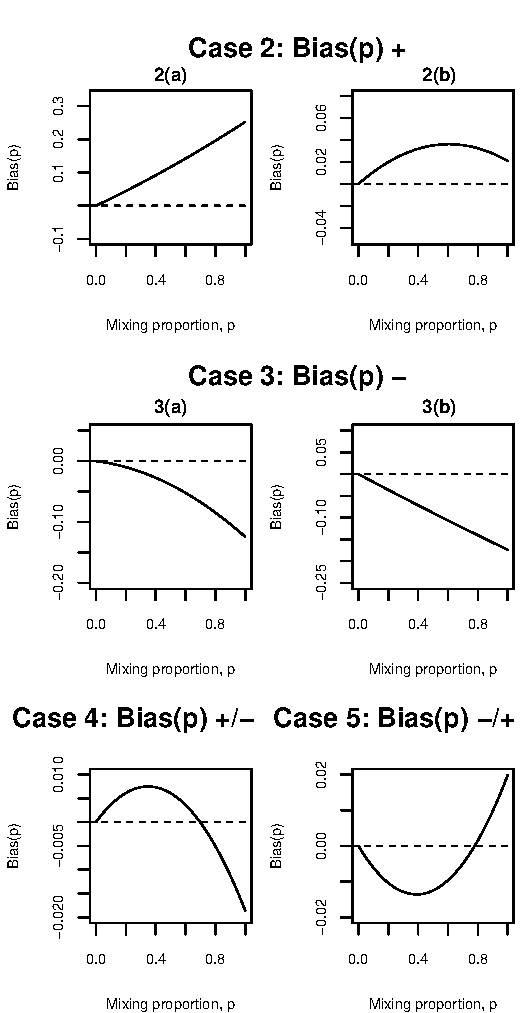
\includegraphics{images/tau_MO_graphs.pdf}
    %\caption{Possible scenarios for bias in Tau for a mixture of Marshall-Olkin distributions. These scenarios were produced using the parameter values in Table \ref{tab:tau}.}
    \caption{Using the values from Table \ref{tab:tau}, these are the possible scenarios for bias in Tau for a mixture of Marshall-Olkin distributions.}
    \label{fig:tauCases}
\end{figure}
\begin{figure}
    \centering
    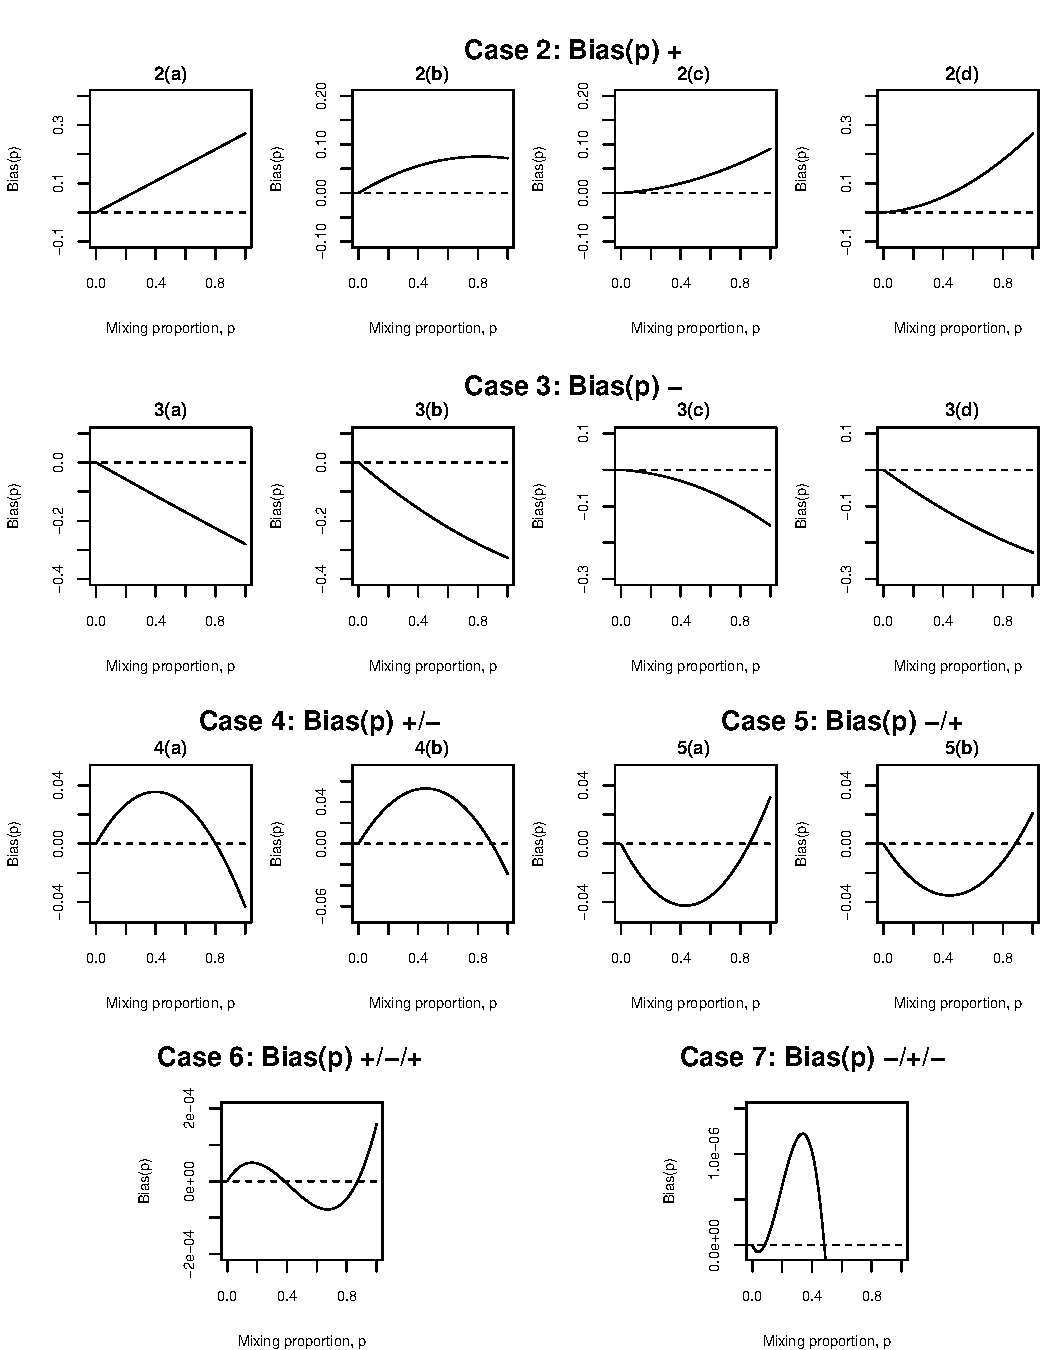
\includegraphics[scale=0.8]{images/rho_MO_graphs.pdf}
    %\caption{Possible scenarios for bias in Rho for a mixture of Marshall-Olkin distributions. These scenarios were produced using the parameter values in Table \ref{tab:rho}.}
    \caption{Using the values from Table \ref{tab:rho}, these are the possible scenarios for bias in Rho for a mixture of Marshall-Olkin distributions.}
    \label{fig:rhoCases}
\end{figure}